%=====================================================================
%  SHARED PREAMBLE — Quantitative Reasoning LAB 413 Beamer theme
%  Paste this block VERBATIM at the top of every LabN_beamer.tex
%  (keep each deck self-contained; do NOT \input this file).
%  Compile: pdflatex LabN_beamer.tex   (run twice for footline counters)
%=====================================================================
\documentclass[aspectratio=169,11pt]{beamer}

\usepackage[utf8]{inputenc}
\usepackage[T1]{fontenc}
\usepackage{lmodern}
\usepackage{amsmath,amssymb}
\usepackage{graphicx}
\usepackage{booktabs}
\usepackage{tcolorbox}
\tcbuselibrary{skins}

\usetheme{default}
\usecolortheme{default}
\useinnertheme{circles}

\definecolor{qrnavy}{RGB}{20,44,90}
\definecolor{qrblue}{RGB}{38,80,150}
\definecolor{qrgray}{RGB}{90,95,105}
\definecolor{qrlight}{RGB}{234,239,247}
\definecolor{qrred}{RGB}{190,60,60}

\setbeamercolor{structure}{fg=qrnavy}
\setbeamercolor{frametitle}{fg=white,bg=qrnavy}
\setbeamercolor{title}{fg=qrnavy}
\setbeamercolor{block title}{fg=white,bg=qrblue}
\setbeamercolor{block body}{bg=qrlight}
\setbeamercolor{itemize item}{fg=qrblue}
\setbeamercolor{itemize subitem}{fg=qrblue}
\setbeamerfont{frametitle}{series=\bfseries}
\setbeamertemplate{navigation symbols}{}

\setbeamertemplate{frametitle}{%
  \nointerlineskip
  \begin{beamercolorbox}[wd=\paperwidth,ht=3.2ex,dp=1.2ex,leftskip=0.3cm]{frametitle}%
    \strut\insertframetitle\strut
  \end{beamercolorbox}%
}

% Footline: course | lab N | slide number  (edit "Lab N" per deck)
\newcommand{\labnum}{Lab 2}   % <-- SET THIS to the lab number, e.g. \renewcommand{\labnum}{Lab 3}
\setbeamertemplate{footline}{%
  \leavevmode%
  \hbox{%
    \begin{beamercolorbox}[wd=.5\paperwidth,ht=2.4ex,dp=1ex,leftskip=.3cm]{author in head/foot}%
      \usebeamerfont{author in head/foot}\color{qrgray}\small Quantitative Reasoning -- LAB 413%
    \end{beamercolorbox}%
    \begin{beamercolorbox}[wd=.5\paperwidth,ht=2.4ex,dp=1ex,rightskip=.3cm]{title in head/foot}%
      \usebeamerfont{title in head/foot}\color{qrgray}\small\hfill \labnum \quad\insertframenumber\,/\,\inserttotalframenumber%
    \end{beamercolorbox}}%
}

% Number badge (01, 02, ...) used on concept slides:  \numbadge{01}
\newtcbox{\numbadge}{on line,boxsep=2pt,left=4pt,right=4pt,top=2pt,bottom=2pt,
  colback=qrnavy,colframe=qrnavy,fontupper=\bfseries\color{white},arc=2pt}

% Key-concepts callout:  \begin{keybox} ... \end{keybox}   or  \begin{keybox}[Scenario] ...
\newtcolorbox{keybox}[1][Key Concepts]{colback=qrlight,colframe=qrnavy,
  fonttitle=\bfseries,title={#1},coltitle=white,arc=2pt,left=4pt,right=4pt,
  top=3pt,bottom=3pt,boxrule=0.6pt}

%---------------------------------------------------------------------
%  Title data
%---------------------------------------------------------------------
\title{\bfseries Describing Data \& Relationships}
\subtitle{Week 2--3 Recap \textbullet\ Lab 2}
\author{Instructor: Subin Na}
\institute{Quantitative Reasoning -- LAB 413}
\date{September 10, 2025}

\begin{document}

%---------------------------------------------------------------------
%  Title slide
%---------------------------------------------------------------------
{\setbeamertemplate{footline}{}
\begin{frame}
  \vfill
  {\color{qrgray}\small Quantitative Reasoning -- LAB 413}\\[0.6em]
  {\usebeamerfont{title}\color{qrnavy}\huge\bfseries Describing Data\\[0.15em]\& Relationships\par}
  \vspace{0.4em}
  {\color{qrblue}\large Week 2--3 Recap \ \textbullet\ \ Lab 2}\par
  \vspace{1.6em}
  {\color{qrgray} Instructor: \textbf{Subin Na} \hfill September 10, 2025}
  \vfill
\end{frame}
}

%---------------------------------------------------------------------
%  Today's Plan
%---------------------------------------------------------------------
\begin{frame}{Today's Plan}
  \begin{columns}[T]
    \begin{column}{0.5\textwidth}
      \textbf{\color{qrnavy}1. Week 2--3 Recap}
      \begin{itemize}
        \item Measures of Center
        \item Spread of Data
        \item Visualizing Distributions
        \item Standardization (Z-scores)
        \item Correlation
      \end{itemize}
    \end{column}
    \begin{column}{0.5\textwidth}
      \phantom{\textbf{x}}
      \begin{itemize}
        \item Linear Regression
        \item Least Squares Regression
      \end{itemize}
      \vspace{0.8em}
      \textbf{\color{qrnavy}2. RStudio Practice}
      \begin{itemize}
        \item Data frames, plots, \texttt{ggplot2}
        \item Transformation, correlation, regression
      \end{itemize}
    \end{column}
  \end{columns}
\end{frame}

%---------------------------------------------------------------------
%  01 Measures of Center
%---------------------------------------------------------------------
\begin{frame}{\numbadge{01}\ \ Measures of Center}
  \begin{keybox}
    \begin{itemize}
      \item \textbf{Mean} = arithmetic average --- \emph{sensitive} to outliers.
      \item \textbf{Median} = midpoint --- \emph{resistant} to outliers.
      \item When distributions are symmetric $\Rightarrow$ mean $\approx$ median.
    \end{itemize}
  \end{keybox}
  \vspace{0.5em}
  \begin{columns}[T]
    \begin{column}{0.5\textwidth}
      \textbf{\color{qrnavy}Incomes} $= [40k, 45k, 50k, 55k, 1M]$
      \begin{itemize}
        \item Mean $\approx 238k \Rightarrow$ does not represent most people!
      \end{itemize}
    \end{column}
    \begin{column}{0.5\textwidth}
      \textbf{\color{qrnavy}Test scores} $= [65, 70, 75, 80, 85]$
      \begin{itemize}
        \item Mean $= 75$, \quad Median $= 75$
      \end{itemize}
    \end{column}
  \end{columns}
\end{frame}

%---------------------------------------------------------------------
%  02 Spread of Data
%---------------------------------------------------------------------
\begin{frame}{\numbadge{02}\ \ Spread of Data}
  \begin{itemize}
    \item \textbf{Quartiles:} split the data into four equal parts.
    \item \textbf{IQR} $(Q_3 - Q_1)$: the ``middle spread'' where most of the data sits.
    \item \textbf{Five-number summary:} min, $Q_1$, median, $Q_3$, max.
    \item \textbf{Standard deviation (SD):} on average, how far the values are from the mean.
    \item \textbf{Outliers:} a common rule is anything more than $1.5 \times \text{IQR}$.
  \end{itemize}
\end{frame}

%---------------------------------------------------------------------
%  03 Visualizing Distributions (1) - boxplots & histograms  (EMBED)
%---------------------------------------------------------------------
\begin{frame}{\numbadge{03}\ \ Visualizing Distributions (1)}
  \begin{itemize}
    \item \textbf{Boxplots} $\rightarrow$ visualize the five-number summary (min, $Q_1$, median, $Q_3$, max).
    \item \textbf{Histograms} $\rightarrow$ distribution shape (bins).
  \end{itemize}
  \vspace{0.3em}
  \begin{columns}[c]
    \begin{column}{0.54\textwidth}
      \centering
      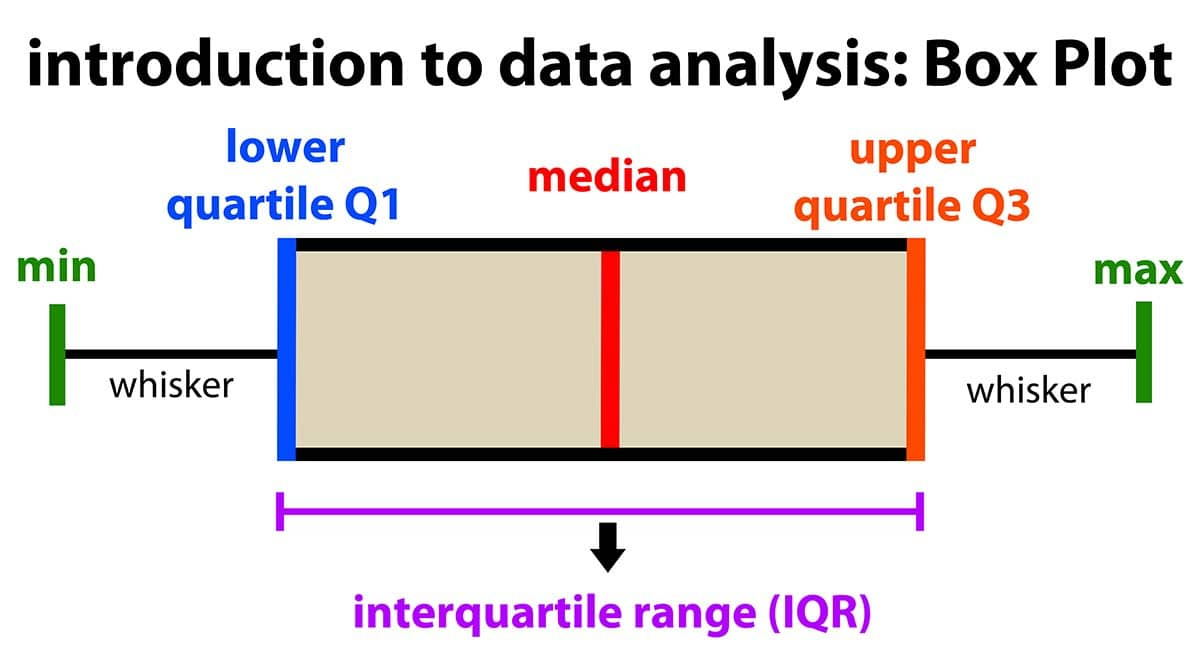
\includegraphics[width=\textwidth]{figures/s05_2_5.9x2.6.jpg}
    \end{column}
    \begin{column}{0.44\textwidth}
      \centering
      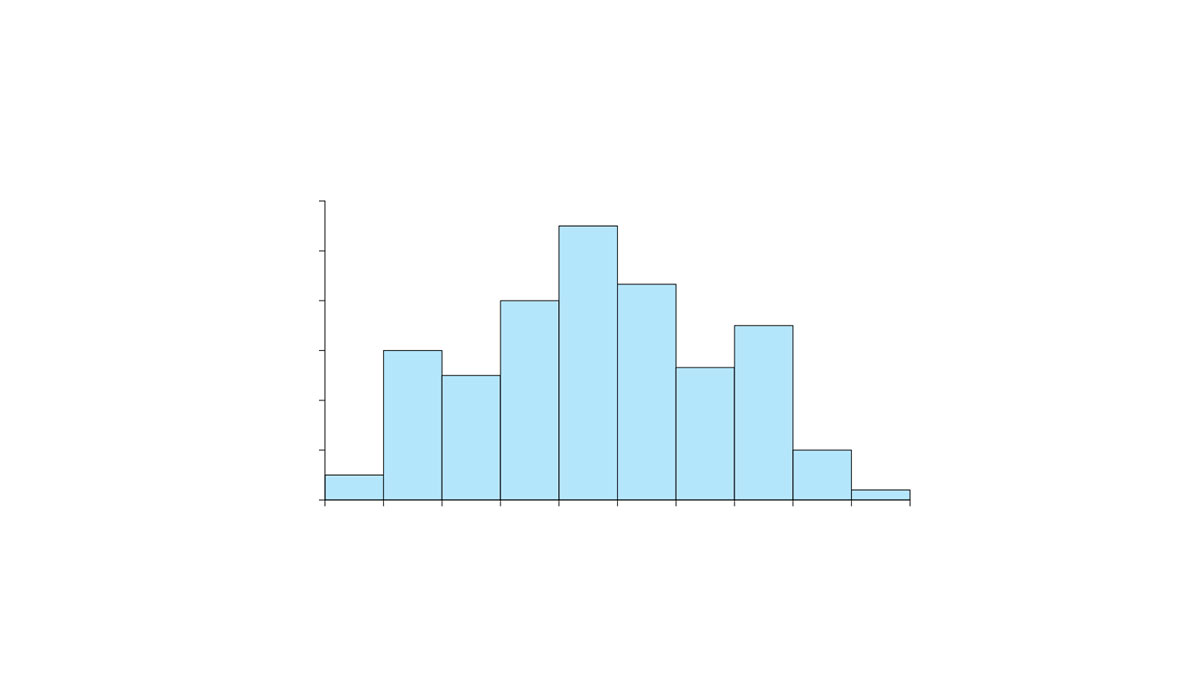
\includegraphics[width=\textwidth]{figures/s05_3_4.7x2.5.jpg}
    \end{column}
  \end{columns}
\end{frame}

%---------------------------------------------------------------------
%  03 Visualizing Distributions (2) - normal curve  (EMBED)
%---------------------------------------------------------------------
\begin{frame}{\numbadge{03}\ \ Visualizing Distributions (2)}
  \begin{itemize}
    \item \textbf{Density curves / Normal distribution:} bell-shaped, symmetric, unimodal.
    \item \textbf{68--95--99.7:} rule for normal distributions.
  \end{itemize}
  \vspace{0.3em}
  \begin{center}
    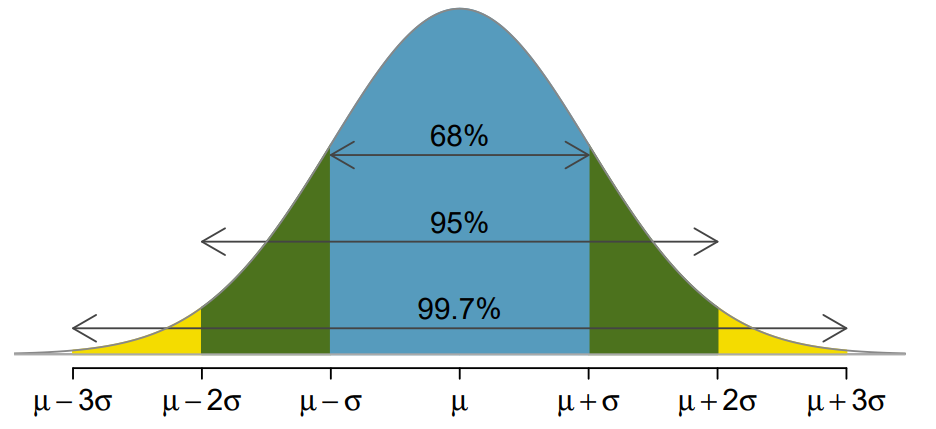
\includegraphics[width=0.66\textwidth]{figures/s05_1_6.8x3.1.png}
  \end{center}
\end{frame}

%---------------------------------------------------------------------
%  04 Standardization (Z-scores)  (RECREATE formula)
%---------------------------------------------------------------------
\begin{frame}{\numbadge{04}\ \ Standardization (Z-scores)}
  \begin{keybox}
    A \textbf{z-score} says how many standard deviations a value is from the mean,
    transforming different units into a common scale.
  \end{keybox}
  \vspace{0.6em}
  \begin{equation*}
    \text{z-score of } x_i \;=\; \frac{x_i - \text{mean of } x}{\text{standard deviation of } x}
      \;=\; \frac{x - \mu}{\sigma}
  \end{equation*}
  \vspace{0.4em}
  \begin{itemize}
    \item Interpret as how many SDs from the mean.
    \item Useful for \textbf{comparing across variables}.
  \end{itemize}
\end{frame}

%---------------------------------------------------------------------
%  05 Correlation (1) - concept
%---------------------------------------------------------------------
\begin{frame}{\numbadge{05}\ \ Correlation (1)}
  \begin{keybox}
    A number that tells you how two variables move together --- it measures
    \textbf{linear association} ($r$ between $-1$ and $1$).
  \end{keybox}
  \vspace{0.6em}
  \begin{itemize}
    \item Positive $r \rightarrow$ variables move \textbf{together}.
    \item Negative $r \rightarrow$ variables move in \textbf{opposite} directions.
    \item $r = 0 \rightarrow$ no linear relationship.
  \end{itemize}
\end{frame}

%---------------------------------------------------------------------
%  05 Correlation (2) - scatterplot grid  (EMBED)
%---------------------------------------------------------------------
\begin{frame}{\numbadge{05}\ \ Correlation (2)}
  \begin{center}
    The best way to see correlation is with a \textbf{scatterplot!}
  \end{center}
  \vspace{0.2em}
  \begin{center}
    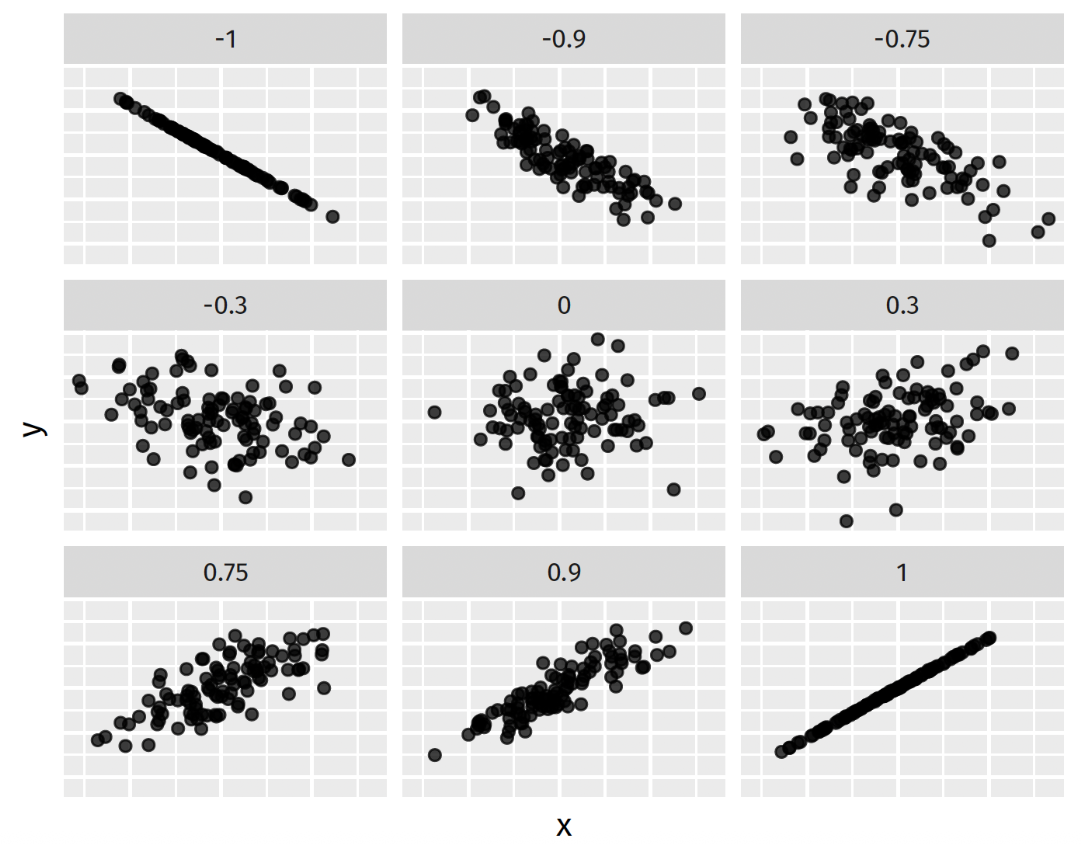
\includegraphics[height=0.72\textheight]{figures/s08_1_8.2x6.4.png}
  \end{center}
\end{frame}

%---------------------------------------------------------------------
%  06 Linear Regression  (RECREATE equation + EMBED diagram)
%---------------------------------------------------------------------
\begin{frame}{\numbadge{06}\ \ Linear Regression}
  \begin{keybox}
    Draw the \textbf{best-fitting line} through the data to predict $Y$ from $X$.
  \end{keybox}
  \vspace{0.3em}
  \begin{equation*}
    Y_i \;=\; \underbrace{\alpha}_{\text{intercept}} \;+\;
      \underbrace{\beta}_{\text{slope}} \cdot X_i \;+\;
      \underbrace{\epsilon_i}_{\text{error term}}
  \end{equation*}
  \vspace{0.2em}
  \begin{columns}[c]
    \begin{column}{0.5\textwidth}
      \small
      \begin{itemize}
        \item \textbf{Intercept} ($\alpha$): value of $Y$ when $X = 0$.
        \item \textbf{Slope} ($\beta$): change in $Y$ per one-unit change in $X$.
        \item \textbf{Residuals:} prediction errors.
      \end{itemize}
    \end{column}
    \begin{column}{0.5\textwidth}
      \centering
      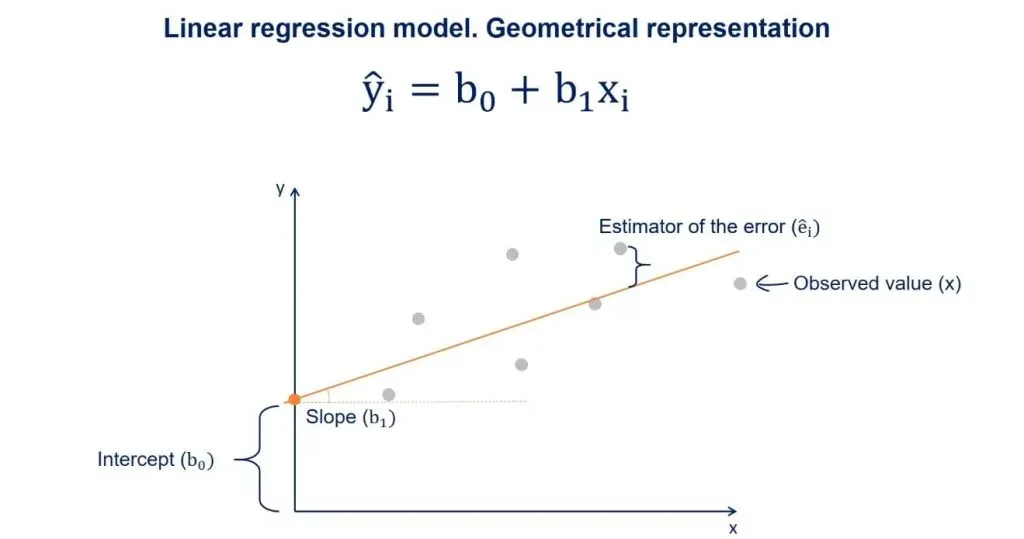
\includegraphics[width=\textwidth]{figures/s09_2_9.7x5.2.png}
    \end{column}
  \end{columns}
\end{frame}

%---------------------------------------------------------------------
%  07 Least Squares Regression  (EMBED)
%---------------------------------------------------------------------
\begin{frame}{\numbadge{07}\ \ Least Squares Regression}
  \begin{columns}[c]
    \begin{column}{0.48\textwidth}
      \begin{itemize}
        \item Find the line that minimizes the \textbf{sum of squared residuals (SSR)}.
        \item The best-fit line balances errors above and below the line $\Rightarrow$
              overall error is minimized!
      \end{itemize}
      \vspace{0.4em}
      \begin{tcolorbox}[colback=qrlight,colframe=qrnavy,arc=2pt,boxrule=0.6pt]
        \centering R function:\\[0.2em]
        \texttt{lm(y \textasciitilde\ x, data = mydata)}
      \end{tcolorbox}
    \end{column}
    \begin{column}{0.52\textwidth}
      \centering
      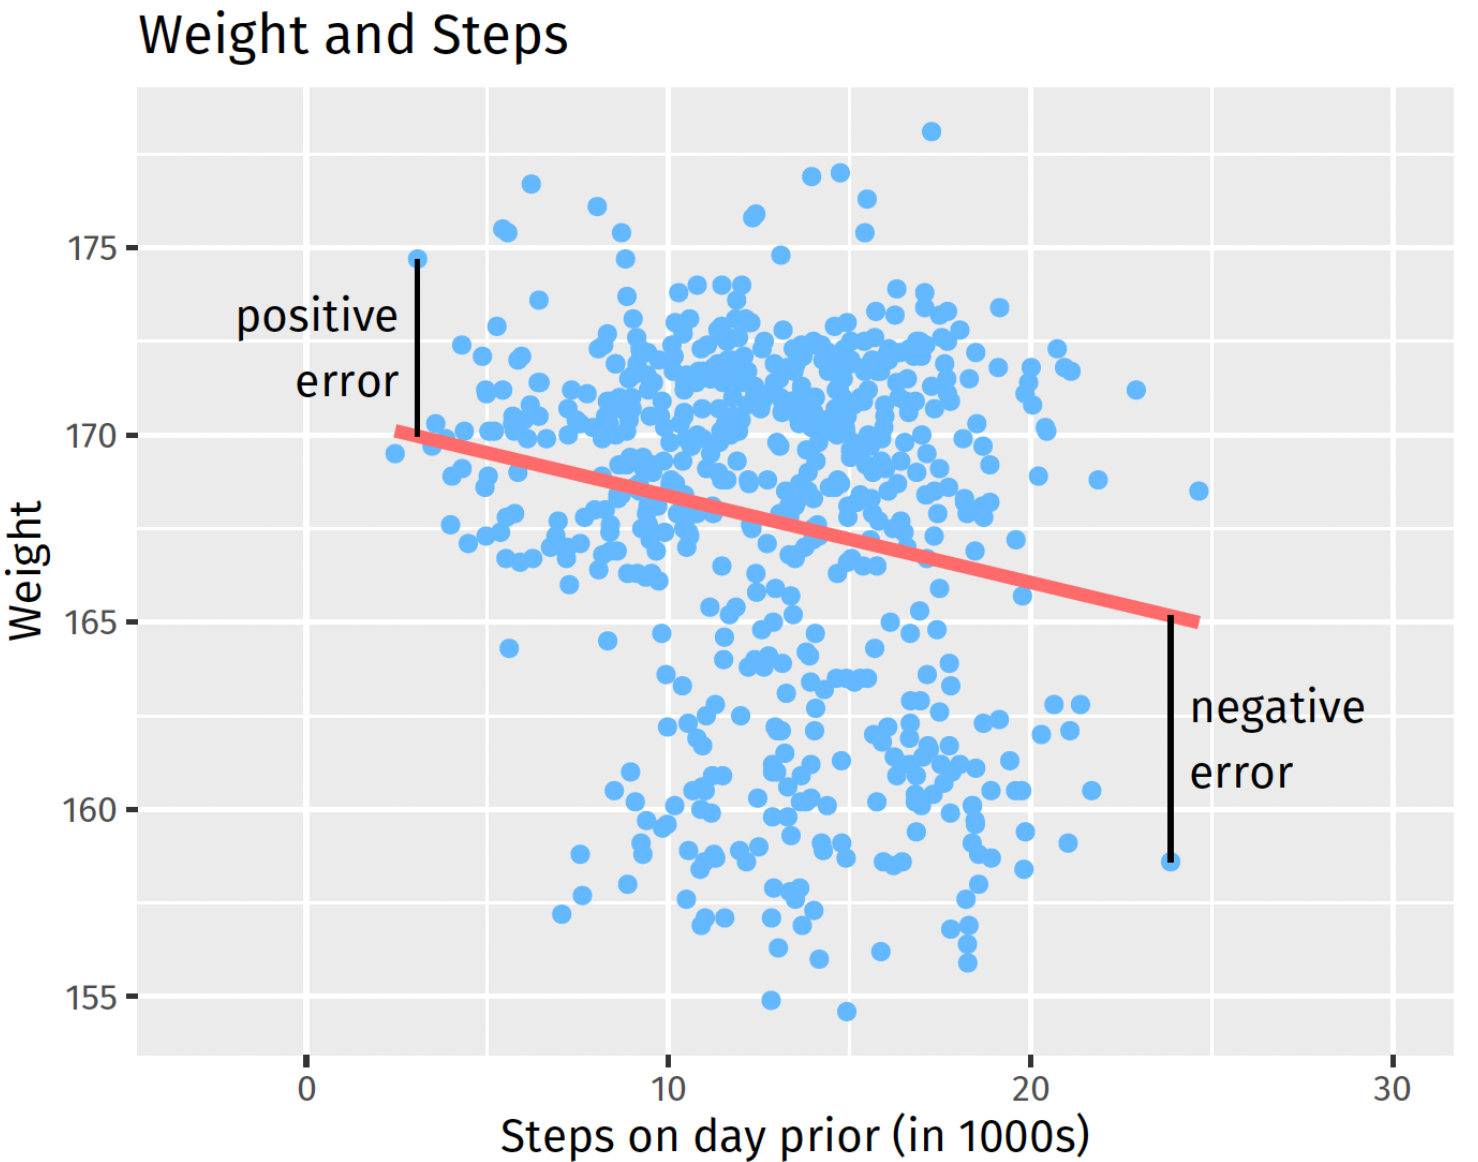
\includegraphics[width=\textwidth]{figures/s10_1_8.1x6.3.png}
    \end{column}
  \end{columns}
\end{frame}

%---------------------------------------------------------------------
%  Transition to RStudio
%---------------------------------------------------------------------
{\setbeamertemplate{footline}{}
\begin{frame}
  \vfill
  \centering
  {\color{qrnavy}\Huge\bfseries RStudio Practice}\\[0.8em]
  {\color{qrblue}\large Visualization, Transformation, Correlation \& Regression}\\[0.8em]
  {\color{qrgray}\small
    \texttt{summary()} for descriptive stats \ \textbullet\ \ \texttt{ggplot2} for plots\\[0.2em]
    \texttt{cor()} for correlation \ \textbullet\ \ \texttt{lm()} for regression}\\[0.6em]
  {\color{qrgray} See \texttt{Lab2.Rmd} / \texttt{Lab2\_0910.R}}
  \vfill
\end{frame}
}

\end{document}
